\DailyTitle{6264 Log (Septemper 30, 2010)}

\DailySection{Goals}

\begin{enumerate}
\item Go through vecbos meetings in september
\item Go through Hcal meetings in september
\item Move the logbook to subversion
\item Make a list of things to do for the candle note
\end{enumerate}

\DailySection{Summary List}

\begin{enumerate}
\item Skimmed through vecbos meetings in espace and V+Jet meetings
\item Skimmed through hcal WG meetings and DPG meetings
\item Moved logbook to subversion
\item Update VecbosApp to newest version, test run on the current muon list (up to run 144114).  No obvious problem spotted.
\end{enumerate}

\DailySection{Go through vecbos meetings in September}

\DailySubSection{Espace meetings}

\begin{enumerate}
\item September 8, "Thresholds" by Maria Spiropulu.   Default value: CaloJet 30, UncorrectedCalo 20, Track 15, PF 30
\item September 8, "Lucas Fit" by Lukas Vanelderen.
   \begin{enumerate}
   \item Fit MT for W, t+X, other
   \item Fix shape to MC for W, t+X, and float the other
   \item "W and top+X separated well and unbiassed from other"
   \item Fit W+LF vs. W+HF with t+X, and use the HF fraction from MC to recover W yield
   \end{enumerate}
\item September 15, "btag" by Lukas Vanelderen.  Control sample for HF from data.  Need to read about b-tagging algorithms.
\item September 15, "Vecbos Meeting" by Matthias Ulrich Mozer.  Revisit uncertainties on AlphaL and AlphaR.
   \begin{enumerate}
   \item Traditional fit: fix alpha to best known value, and redo fit with different alpha to get uncertainty
   \item Nuisance parameter: constrain alpha by a gaussian centered at the best known value.
   \item 7-fit plot.
   \end{enumerate}
\item September 22, "Vecbos Meeting".  "W and Z + jets" by E. di Marco in General EWK meeting.
\item September 22, "Vecbos Meeting".  Lukas updated results on WJet fit.
\item September 22, "Vecbos Meeting".  Will Reece updated on trigger efficiencies.
\item September 29, "W fit strategy, flavor part" by Lukas Vanelderen.
Estimate PDF from b-tag variables from control samples for t+X and W+LF.  Seems to have problem in the 2Jet bin.
\end{enumerate}

\DailySubSection{V+Jet meetings}

\begin{enumerate}
\item September 7.  Lukas on fit strategy in W+Jets (sane as the one in espace).  Z candle analysis status report (with toys).
\item September 21, "Introduction on Zbb issues and current plans" by Alexandre Nikitenko.  Z+b is similar to H+b
\item September 21, "Task list overview" by Vitaliano Ciulli and Ilaria Segoni.
\item September 28, "Report on Zbb analysis" by Anne-Marie Magnan.
\item September 28, "Report on Zb(b) analysis" by Natalie Heracleous.
\item September 28, "Update on Z(ee)+jets and W(enu) +jet studies" by Sarah Malik. (....)
\item September 28, "Status on PFlow Z+Jets Analysis" by Anil Pratap Singh.
\end{enumerate}

\DailySection{Go through Hcal meetings on noise}

\DailySubSection{Hcal Noise WG}

\begin{enumerate}
\item September 9, "HF Flags in 3\_8 (slides for Maria)".  Some notes on HF reconstruction and flagging.
\item September 9, "Isolated Noise Filtering" by John Paul Chou.  Summary of the isolation-based noise filter.  Performance on ttbar and Ztautau.
Suggests going on to JetID.  Reviewed reconstruction chain.
\item September 9, "HPD Pulseshape Discriminators" by Jason St. John.  Included HE.  MC shape needs work.
\item September 9, "Hits in a Jet" by Hongxuan Liu.  Good hits and PMT window hit could overlap.
\item September 9, "HBHE Timing and Noise Studies" by Phil Dudero.  Derive time envelope from collisions.
Plots for time envelope with/without low energy hits as well as square filter (energy independent).
\item September 9, "Impact on MET due to ECAL masked/dead cells" by Hongxuan Liu.  Jet response 2\% quantile map.  Holes correspond to dead cells.
Jet energy recovery algorithm.
\item September 23, "Isolated Noise Filter: Performance" by John Paul Chou.  Update his filter to be used as a hit cleaner and not a event filter.
\item September 23, "HBHE Timing and Noise Studies" by Phil Dudero.  Some error/problem two weeks ago.  Updated square filter results.
\end{enumerate}

\DailySubSection{Hcal DPG}

Note: Talks that have nothing to do with noise are omitted here.

\begin{enumerate}
\item September 13, "HCAL QIE Offsets" by a list of people.  The new setting is consistent with old setting (with a overall constant shift) for HB and HE.
\item September 13, "HCAL Noise" by Maria.  A summary to be used in Bodrum.
\item September 27, "TP Energy Scale" by Patrick Tseng.  He recalibrated and checked TP energy.
\item September 27, "QIE hardware offset and time reco" by Pawel de Barbaro.  Validated new QIE settings.  Overall good.  Time spread is smaller.  Some channels (not many) are off.
\item September 27, "Precise time correction" by Jeremiah Mans.  An independent analyses to derive time corrections.  Compared with those from Pawel et al. and looked at channels that disagree.
\item September 27, "An Isolated HB/HE Noise Filter" by John Paul Chou.  Same talk as in Hcal noise WG.
\item September 30, "Phi calibration of HB, HE - initial results" by Igor Vodopiyanov.  Intercalibration using non-ZS data.  Not clear from the presentation what "E1" is.
\end{enumerate}

The QIE hardware timing offset is adjusted since runs 146XXX! 

\DailySection{Updating VecBosApp to newest version and test run on data (2.66/pb)}

\begin{enumerate}
\item Everything went fine on cvs update and merging versions.
\item Test run on ZJetsMADGRAPH sample, all jobs finished successfully, though castor was busy for one job.  Rerun does the job.
\item Copying from castor back to local disk gives ". : Invalid argument".  Maybe castor was extremely busy.
\item ps. the error means that disk quota was exceeded.
\item No problem spotted in ZJetsMADGRAPH sample from the QM plots.
\item Test run on current dataset (up to run 144114, 2.66/pb reported).  While submitting jobs, encountered one instance of
"LSF js on lxbsp0901.cern.ch: LFS js: no AFS token" error.  It doesn't seem to be related to the updating of VecBosApp.
It doesn't seem to be affecting anything either.  Jobs are successful.
\item The castor-friendly safety sleep time (10s) is getting annoying now that there is more statistics.  Let's try to reduce it to 3 seconds.
\item Data looked OK at first glance.
\item The mass of any two global muons looks nice, see figure \ref{Figure_6264DiGlobalMuonMass_DataAll}.
\end{enumerate}

\begin{figure*}
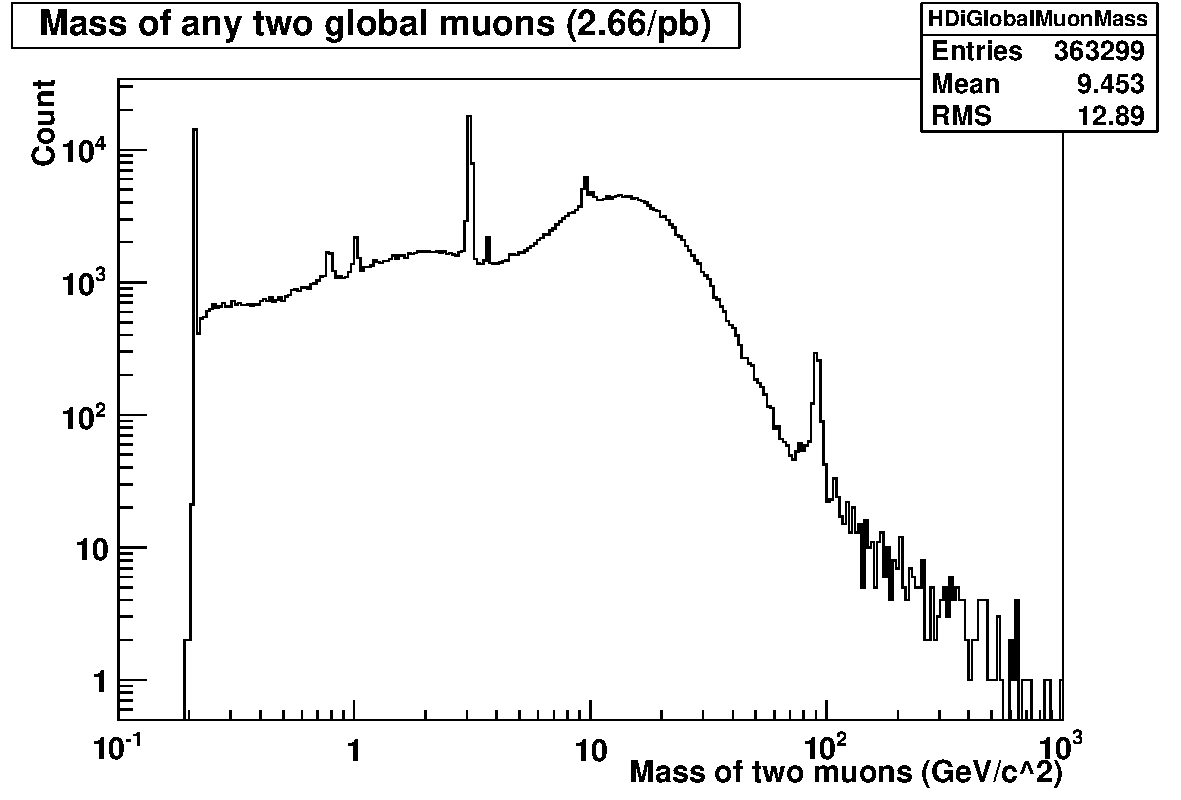
\includegraphics[width=120mm]{DailyLog/6264/6264DiGlobalMuonMass_DataAll.pdf}
\caption{Mass of any two global muons from all processed data so far (up to run 144114).  Peaks from right to left are speculated to be
Z (\tweakedtilde90), Upsilon family (\tweakedtilde10), J/Psi(1s, 2s) (\tweakedtilde3), phi (\tweakedtilde1), rho (0.7\tweakedtilde0.8), and muonium (\tweakedtilde0.2).
(ps. The last one was just kidding.  It's probably from doubly reconstructed ghost muons.  Though further investigation is needed.)}
\label{Figure_6264DiGlobalMuonMass_DataAll}
\end{figure*}

\DailySection{Meeting notes}

\DailySubSection{Caltech group meeting}

\begin{enumerate}
\item There is some narrow peak discovered (!?)
\item Maria: the comment system needs to be rethought.  Actual commitment is needed.
Comments on physics, not styles.
\item Artur gave a presentation on the recent drama on Hcal.  Accidental unmasking of hcal bad channels,
severity level in HLT
\item Piotr reports on the peak of opposite-sign dimuons around 244 GeV.
\item Update from Jan.  Z->mumu vs. mumu+gamma, Energy scale of photon.
\item Action items for next Tuesday to be emailed out by Dorian
\end{enumerate}

\DailySection{Reflection}

To fully understand hcal noise, we need to have real categories (instead of the simplistic ion/hpd/rbx picture),
and monitor the change over time to obtain a control sample estimate of the amount of noise of each type for all RBXs.


\DailySection{Goals for next work day}

\begin{enumerate}
\item Sort out goals for Hcal noise line
\item Make sure how prescale works with multiple triggers
\item Make a list of to-do items for candle analysis
\item Review/summarize progress so far on pulse shape variables
\item Check strategy on Z shape fit, find out ways to contrain RooFormulaVar
\end{enumerate}


